\chapter{Layout of the Program}\label{layout-of-theprogram}

\section{Objectives}
In this chapter, you are going to learn how to lay out your program
following a pattern that will make your code easier to understand, to
maintain and to share. Normally, you should have defined the structure
of the program before you start writing code. However, development is
not always linear and projects that begin small end up controlling very
complex experiments. Sometimes you can already know how the future
looks, what experiments you may want to perform in a year from now or
even more. In any case, building on top of a solid foundation allows you
to be future proof.

In this chapter, You will learn about some common design patterns and
general ideas that are used in the long run. What you are going to learn
in this chapter is a collection of best practices, which doesn't mean
you have to follow them to the letter, but they are a very good starting
point. You will learn about the {MVC} design pattern, which will allow
you to separate different elements of your code into reusable
containers. Moreover, you will create a specific folder structure that
will enable to use code shared by others. The {MVC} design pattern forms
a layered structure, exactly in sync with the ideas that we have exposed
when discussing the \emph{onion principle} for development.

\section{Introduction}
Computer programs are meant to be a solution to a more or less complex
problem. It seems unlikely today that anybody would invert a matrix by
hand or with a calculator. Nor to imagine that somebody would plot a
complicated function with pen and paper. Several packages exist to solve
those needs, from Python to Matlab to Origin. In the same fashion, the
complexity of experiments is such that it is impossible to control all
the needed variables by hand. Even in simpler experiments, there will
always be a computer responsible for acquiring data, saving it, and many
other things.

Developing a computer program for controlling an experiment is not a
trivial task. One has to consider the limits of the devices, acquisition
rates, conditions for closing a shutter or switching off the power. On
top of all that, one has to write programs that most likely are going to
be used by others, and that can be developed further on by another
person. It doesn't make sense to write software today that will be
obsolete next week just because few parameters of the
experiment changed.

To address these concerns, there are few techniques that a developer can
follow in order to achieve a high degree of productivity and, at the
same time, producing software that can be enhanced later on. The idea of
establishing best practices is not increasing the burden of developing
software, but to streamline the process. The cornerstone of every great
program is to have a design pattern that can be followed by all the
developers. Therefore, when developing software for controlling a setup
we have to keep an eye on different considerations:

\begin{itemize}
\item What you develop should be readable by current and future colleagues
\item It should be easy to add solutions developed by others
\item The program should allow exchanging devices that achieve the same goal (i.e. oscilloscopes of different brands, etc.)
\item The code developed in one context has to be available in other contexts (i.e. in other experiments)
\end{itemize}

As you can see from the list above, it is very desirable to be able to
reuse code, not only within the same lab with the same colleagues but
also to use code that was developed in other institutions. On the other hand, you would like that your own code can be reused. This will help you save time when you move on to other projects, but it will also give you a specific place in a community, since you are giving something back. Reusing code is not only a matter of saving time, it also empowers collaboration between different labs. Reusing code needs that some standards are specified, in such a way that another person can easily include the code in their projects. In the previous chapter we started working in this direction when we defined a class for controlling the device and not a plain script.

The problem with rules is that they are normally percieved as an obstacle in a developers roadmap. After a long time of trial and error, we have come up with some general rules that don't increase the overhead for a developer willing to find a solution to a specific problem. At the same time, the rules are such that when the program gains complexity it will allow different persons to collaborate seemlesly, and it will generate a base that can be continuously expanded over the long term. Moreover, the rules that we are going to discuss in this chapter were developed in such a way that the end program will be welcoming to new developers willing to contribute and to learn from the existing code. 

\section{The MVC design pattern}\label{the-mvc-designpattern}
\begin{center}
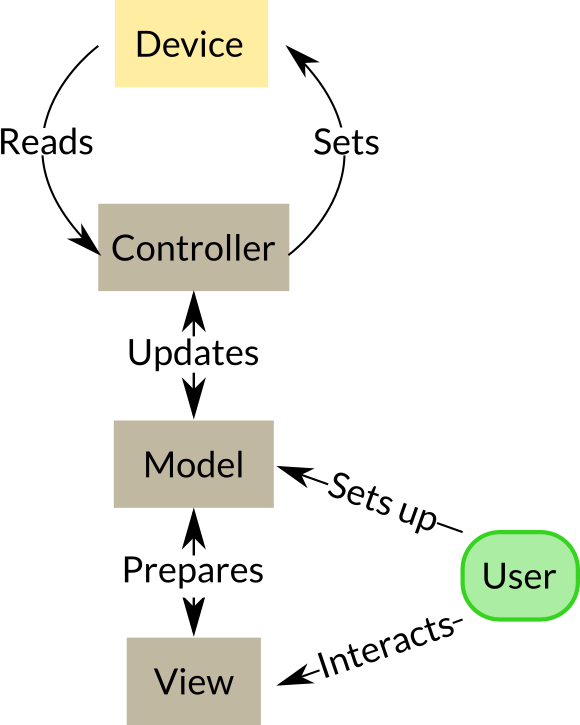
\includegraphics{images/Chapter_04/MVCs.png}
\end{center}

A design pattern is nothing more than a set of rules that determine where different parts of the code are going to be placed and how are they going to interact with each other. One of such patterns is called the Model-View-Controller, or MVC for short. When you work with devices in the lab, there is an extra layer that most computer programs lack, which is the interaction with the real world through specific devices. That is why we decided to nickname the pattern MVCs, with the s for \emph{science}. Let's see what each component of the MVC is about. 

A \emph{Controller} can also be called \emph{the driver}, which is responsible for communicating with the devices. It can be a Python class you developed yourself such as the one we did in the previous chapter, but it can also be a Python package developed by someone else. The latter scenario is the case in which manufacturers provide the drivers themselves, such as PyPylons from Basler, or the NI-DAQmx bindings for Python. The driver has to reflect the capabilities of the device, nothing less and nothing more. For example, if a device is able to acquire just a data point at a time, the
driver shouldn't include a function for acquiring an array of data using a loop. We briefly discussed this in the previous chapter. Whatever belongs to the logic that a user imposes belongs to Model component. 

The \emph{Model} is where all the logic is defined. In the models, you are going to define how you are going to use a device for your own experiment. A clear example would be the introduction of units. The device from the previous chapter takes only integer values as inputs. If you would like to transform that input to voltages, you could do it in the model for the device. Moreover, one of the analog inputs is measuring volts, but they can be translated to a current. This is very specific to our experiment and thus the option shouldn't be hardcoded in the driver, but it has to be an option in the model. The main advantage of splitting \emph{Controllers} and \emph{Models} is that it becomes simple to upgrade or replace a device. You will need to update the \emph{Model} in order to reflect the new options of the device, but the logic of the experiment is left intact. 

Splitting the Model from the Controller will look like extra work at the beginning without a clear gain. The main advantages appear when you are using a driver developed by someone else and when you know you will need to change the devices on your setup. In this book, we work only with one device and in a very simple experiment. Therefore, the advantages of the Model are not going to be evident to inexperienced developers. Once the program you are developing has enough mileage, you will see the payoff of having a clear structure. 

The \emph{View} is, the place where you can locate everything related to how you show data to the user, and how the user can change the parameters of the experiment. In practice, it is the collection of files that build up a Graphical User Interface ({GUI}). Within the {GUI} you will set, for example, the length and delay of the time trace you want to acquire. This information will be passed to the model to acquire the data. You can plot the results back to the user and save them to disk, etc. It is important to note that, in this case, the user interacts through the view with the model and never directly with the controller of a device. It is also important to keep in mind that all the logic of what you are developing should be implemented in the model. For example, if you save the data to files, the procedure to create new filenames should be specified in the Model and not in the View. 

\warning{If you are new to developing code for the lab, it may seem that splitting \emph{Controller} and \emph{Model} is a waste of time. When
you have only one device that you use for only one goal, it may very well be the case. However, when you wish to include code developed by
others or when you want to share your code, it is crucial that you split the capabilities of your device from the logic of your experiment. If
you don't do so, all your code is going to work only when doing just one, very specific, experiment.}

You have to remember that the meaning of \emph{Model}, \emph{View} and \emph{Controller} changes depending on each developer or community. It
is important to note that people developing a web application are not dealing with devices in the real world as developers in the lab do. Therefore, how the {MVC} pattern is used can change from one field to another. Once you understand what each component is, you will very quickly understand where you need to change the code in order to solve a bug or add a new functionality. 

\section{Structure of The Program}\label{structure-of-theprogram}
In the program you are developing in this book, you will follow the {MVC} design pattern quite literally. This means that you have to create
three folders called \emph{Model}, \emph{View} and \emph{Controller}. In the previous chapter you have already developed the driver for the device. Go ahead and move the file \textbf{simple\_daq.py} into the Controller folder.

\exercise{Create a file \textbf{analog\_daq.py} in the Models. Inside the file, define a class called \mintinline{python}{AnalogDaq} and move the methods that you think appropriate from the Controller into the Model.}

In our definition of Model, it is important to make a further distinction. On the one hand, you have models for the devices that you use. In those models you will define things such as units, how to initialize the device, etc. However, experiments often require to perform complex tasks in which several devices are synchronized. When you do an experiment you will need to save the data, or load the configuration from a file. 

\exercise{Create a file in the Models folder, called \textbf{experiment.py}. Define a class called \mintinline{python}{Experiment} and add some methods that you think are going to be useful. You can, for example, add a method for switching on or off the {LED}. You can also add a method for doing a scan of an analog output signal. The methods can be empty, don't worry about making it work, but about the layout. You have to start thinking about the parameters that you need and the order in which every method can be called. For example, you can't save the data if you didn't perform any experiments.}

The View folder is going to require a bit more of work than the other two. However, you can already start thinking about how the user is going
to interact with your program. Most likely, you have already thought that sometimes the {LED} will be plugged into the output channel number 1,
sometimes to channel number 0. You don't want to change the code every time you change where you plugged the LED. The same happens, for example, with the channel you want to monitor, the time delay between steps, etc. All this behavior will be included into the view in the last chapters of the book. 

Now that you have started to split the code into different folders and files, it is important to discuss how can you make programs that use the code avilable in different files. That is colled \emph{importing} and is the focus of the next section. 

\section{Importing modules in Python}
In the previous chapter, we have already seen some lines that look like this:

\begin{minted}{python}
import numpy as np
from time import sleep
\end{minted}

The first one is importing the numpy package, but changing its name to \mintinline{python}{np}. Changing the name makes it easier to work with because you need to type only two letters, \mintinline{python}{np} instead of \mintinline{python}{numpy}. The second line is importing one specific function from a package called \mintinline{python}{time}. It is important to realize that the import process was different in both cases. \emph{Numpy} is a
complex package, with a lot of modules that can be used. The same is true for \emph{time}. However, in the lines above you have imported only the module \emph{sleep} from package \emph{time}. If you want to use it, you can simply do:

\begin{minted}{python}
sleep(1)
\end{minted}

While for using \emph{Numpy}, you will need to specify which module you want:

\begin{minted}{python}
np.random.random(1)
\end{minted}

If you know you only want to use \mintinline{python}{random} from \emph{Numpy}, you can also import and use it like this:

\begin{minted}{python}
 from numpy.random import random
 
 random(1)
\end{minted}

You may wonder why you would import all of numpy is you are just using one of its functions. The name \emph{random} is not defined solely by numpy. Python also provides its own random module. You can import it like this:

\begin{minted}{python}
 import random
\end{minted}

If you needed both \emph{random} functions in the same program, you would have a clash. How would you be sure you are using Numpy's and not Python's function? You may, for example, define your own random function and you would like to be able to choose which one to use and, more importantly, you want to avoid generating an unexpected behavior because of redefining functions without realizing it. 

When working with your own code, you can import different modules in the same way. Open a terminal and navigate to the root folder of the project, i.e. the folder that contains the Model, View, and Controller folders. Start the Python interpreter, and then type:

\begin{minted}{pycon}
>>> import Controller
\end{minted}

Now you have the controller available to use. For example, you can do the following:

\begin{minted}{pycon}
>>> dev = Controller.simple_daq.SimpleDaq('/dev/ttyACM0')
\end{minted}

And you can use the device as you have been using it in the previous chapter. Importing the \emph{Controller} may not be exactly what you
want, because sometimes there are many devices and you need only one. You can specify which module to import, exactly as you have done with
\mintinline{python}{from time import sleep}. To import only the SimpleDaq class, you can do:

\begin{minted}{pycon}
>>> from Controller import simple_daq
>>> dev = simple_daq.SimpleDaq('COM1')
\end{minted}

There are two things important to notice. First, if you change the code of the \emph{SimpleDaq} class and import it again, you won't see those
changes reflected. You should exit from Python and start again. The second thing is that, when you import the controller, you may also start
communicating with the device. This is happening because at the end of the \textbf{simple\_daq.py} file, you have added some lines for actually using
the class. Those lines also get imported and executed. When you import modules, and when you design modules, it is very important being in control of what is going to be executed. You don't want to trigger a measurement just because a user imported your driver. 

To avoid starting the communication with the device when you do \mintinline{python}{import simple_daq}, you have to add one line of code at
the end of the file. It will look like this:

\begin{minted}{python}
if __name__ == "__main__":
    d = SimpleDaq('/dev/ttyACM0')
    print(d.query('IDN'))
    d.write('OUT:CH0:4000')
    input('Press to read value')
    print(d.query('IN:CH0'))
    d.finalize()
\end{minted}

Next time you do \mintinline{python}{import simple_daq}, the code that follows the if statement will not be executed. However, if you run the file  itself by typing \mintinline{bash}{python simple_daq.py}, it will. This is very useful because it allows you to distinguish the two cases, when the file is directly executed and when the file is imported. In many cases, you can use the bottom of the file to show how the class is used or to perform some quick tests. In the code above you can quickly see how to start the communication, query for the serial number, change the analog output, etc.

To understand a bit more about how the \mintinline{python}{if __name__} works and have a clearer picture of the importing procedure in Python, create
a new file called \textbf{dummy\_controller.py} in the \emph{Controller} folder, and paste the following lines of code:

\begin{minted}{python}
print('This is the dummy Controller')

def dummy_example():
    print('This is a function in the dummy Controller')

if __name__ == '__main__':
    print('This is printed only from __main__')
\end{minted}

From the terminal, enter into the Controller folder and type \mintinline{bash}{python dummy_controller.py} The output that you see should be:

\begin{minted}{python}
'This is the dummy Controller'
'This is printed only from __main__'
\end{minted}

What you see is that the entire code got executed but not the function itself. \mintinline{python}{dummy_example} is only defined, but never executed.

\exercise{What do you expect it to happen if you do \mintinline{python}{import dummy_controller}?}

Things are going to be different when you import the file. Open the Python interpreter and type the following:

\begin{minted}{pycon}
>>> import dummy_controller
"This is the dummy Controller"
>>> dummy_controller.dummy_example()
"This is a function in the dummy Controller"
>>> from dummy_controller import dummy_example
>>> dummy_example()
"This is a function in the dummy Controller"
\end{minted}

The first thing you should notice is that what is written at the end never gets executed, meaning that the \mintinline{python}{if} statement is not
\mintinline{python}{True}. This is very useful when we want to have code that works standalone (when we execute it directly, for example) but we don't want to execute those lines if we import it. In the case of the real controller, we wanted to leave some examples at the end to show how it can be used, but when you are importing a class, you don't really want it to start communicating with the device.

The other thing that you should have noticed is that depending on how you import from a file, the first print statement is executed or not. If
you type \mintinline{python}{import dummy_controller}, you will see that the first print statement is there, while if you type \mintinline{python}{from dummy_controller import dummy_example} nothing happens. This is very useful because it means that in the first case you are really executing everything within the file, up to the \mintinline{python}{if} statement. In the latter case, however, you are only getting the specific function you want.

Finally, it doesn't really matter how you imported the dummy controller, the \mint{python}|dummy_example| function will always be available. It can happen that you either have to type \mintinline{python}{dummy_controller.dummy_example()} or simply \mint{python}|dummy_example()| but you will always see the same output. If you were sitting in an outer directory, you would have to do \mint{python}|Controller.dummy_controller.dummy_example()| and it would still work. When working with modules, there is plenty of flexibility on what to do. Bear in mind, however, that the same flexibility comes accompanied by some usage patterns that may not be clear.

Imagine you add a second function to your \mintinline{python}{dummy_controller.py} file, you can import both at the same time by typing
\mint{python}|from dummy_controller import dummy_example, second_function| You could also do \mint{python}|from dummy_controller import *| The
second option, however, is highly discouraged. There are several disadvantages to doing so. First, if you are reading the code and you
see something called \mintinline{python}{second_function} you have no idea where it came from. Also, if the \mintinline{python}{dummy_controller} creates variables, they will appear in your own program, perhaps overriding something you wanted to preserve.

\note{We should establish some naming conventions in order to avoid confusion later on. In Python, any file that defines variables, functions, classes, etc. is called a \mintinline{python}{Module}. The folder that contains modules is called a \mintinline{python}{Package}.}

Working with the imports in Python is sometimes easier than understanding them, especially when trying to pay attention to all the different definitions. The \href{https://docs.python.org/3.6/tutorial/modules.html}{Python Documentation} has a great chapter covering a lot of the ideas here
discussed. Many of the properties and behaviors can be learned by trial and error, though it can be very time consuming and it may lead to unexpected errors.

Perhaps you noticed by now that the way our package is imported and the way \emph{Numpy} is imported is very different. \emph{Numpy} can be
imported regardless of where you have started the Python interpreter. However, our package can only be imported if you are in its own directory. When you perform an \emph{import}, Python searches for modules in specific locations, and once it finds one, it stops searching. \emph{Numpy} is located in one of such folders, but your package is not. One of the ways in which you can let Python know where your package is located is by adding the folder of your package to a system variable called \emph{PYTHONPATH}.

If you are on Windows, you can follow the steps of Chapter 2, when you were dealing with the details of adding environment variables when
installing Python. If you are on Linux, it is enough to run the following command:

\begin{minted}{bash}
export PYTHONPATH=$PYTHONPATH":/path/to/PFTL"
\end{minted}

Remember that you have to change \texttt{/path/to/PFTL} with the full path to the folder where you are keeping your code. After doing that, you will be able to type \mint{python}|from Controller import *| wherever you are in your computer and Python will find the appropriate folder. In Linux, the change is not permanent, you will need to run the line again next time you start the Terminal. There are ways of modifying the environment variables in a permanent way, but it is up to you to find out. There are a lot of tutorials available online, according to your own distribution. 

There is something very important to add to our packages, the
\textbf{\_\_init\_\_.py} file. Sometimes it is important to let Python
know that a specific folder is a package to prevent directories with a
common name, such as \mintinline{python}{string}, from unintentionally hiding valid
modules that occur later, on the module search path. The
\textbf{\_\_init\_\_.py} file can be an empty file, but it can also be
used in smart ways. Normally the \textbf{\_\_init\_\_.py} file can be
used for some initialization. You can create therefore an
\textbf{\_\_init\_\_.py} file within the \emph{Controller} directory and
place the following:

\begin{minted}{python}
from .simple_daq import SimpleDaq

Controller_variable = "var"

print("This is the init of the controller")
\end{minted}

Go back to the root folder, one level up from the Controller folder and
start Python.

\begin{minted}{pycon}
>>> import Controller
"This is the init of the controller"
\end{minted}

It is super simple and clean. If you want to use the \emph{SimpleDaq}
class, you can just type \mintinline{python}{Controller.SimpleDaq}. Moreover, you
should have seen the print statement appearing on your screen. This
means that the \mintinline{python}{Controller_variable} is also available, you can
see it by typing:

\begin{minted}{pycon}
>>> print(Controller.Controller_variable)
"var"
\end{minted}

You could also import only the Controller class or the variable. You
should just do:

\begin{minted}{pycon}
>>> from Controller import Controller_variable
>>> from Controller import SimpleDaq
\end{minted}

How many times do you see the print happening? Interesting, isn't it?
Python takes care of executing the code only once, the first time it
encounters an import statement. We will look again at the
\textbf{\_\_init\_\_.py} file later on. For the time being it is
important that you realize that sometimes things happen within that
file. A lot of code can be executed within the \textbf{\_\_init\_\_.py}
file and therefore you should also look into them when there is
something mysterious that you cannot understand or when you don't find
the file from which an import is happening.

\exercise{Read the Documentation and find a way in which the code
\mintinline{python}{from Controller import *} imports only the \mintinline{python}{SimpleDaq}
class and not the variable we introduced in the \mintinline{python}{__init__.py}
file.}

\section{The Final Layout}\label{the-finallayout}
Now you have a clear separation of your code into Model, Controller, and
View. However, these are not the only folders that you are going to use.
Most likely you will want to provide some examples of how to use your
code, or the documentation for your package. We have also discussed
using text files for the input data, and those files should be located
somewhere, for example within a \emph{Config} folder.

If you create extra folders next to the three main ones, the structure
of the program will start to be polluted. It won't be clear what is part
of the package, what is a user-specific setting, etc. Therefore you need
to create a folder for the main part of the code and next to it the
extra folders that you need. Your folder structure will look like this:

\begin{minted}{text}
├── Docs/
├── Examples/
│   └── Config/
└── PythonForTheLab/
    ├── Controller/
    ├── Model/
    │   ├── daq/
    │   └── experiment/
    └── View/
        └── GUI/
\end{minted}

You can see that there are three folders at the top level, \emph{Docs},
\emph{Examples} and \emph{PythonForTheLab}. The last one is holding the
\emph{Model}, \emph{View} and \emph{Controller}. You can also see that
in the \emph{Model} we have created two separate folders, one for
dealing with the daq and one for dealing with the experiment. If you
followed the steps to add the folder to your Python path variable, it
means that now you can do the following, for example:

\begin{minted}{pycon}
>>> from PythonForTheLab import Controller
\end{minted}

The only missing folder is the one in which we are going to store the
data that we want to pass to the experiment. In this case, you should
consider different scenarios. At this stage, you are the only one
working and using the code, but later on, maybe there are more users.
Or, you are the only developer, but there is more than one user of the
same setup. In any case, when you configure your experiment, you don't
want people to change it, but they should be able to do it
for themselves.

In order to be flexible, the best idea is to provide a folder with
Examples of how to configure your program, or how to generate the
configuration files. These are just examples, aimed at exposing all the
configuration options. However, when you want to run the experiment, you
will do it starting with a different set of files, stored in a
different location.

Let's start simple. In the \emph{Config} folder that lays within the
\emph{Examples} folder, you have to create a file called
\textbf{experiment.yml} to hold all the parameters of the experiment.
Earlier we have decided that the format of the file was {YAML}. If you
are not familiar with the format, it looks like this:

\begin{minted}{yaml}
Experiment:
  name: This is a test Experiment
  range: [1, 10, 0.1]
  list:
   - first Element
   - second Element
\end{minted}

This file is plain text but with a very special structure. {YAML} is
very simple to read and has just a few rules, the most important one is
that the indentation is done with 2 spaces. The choice for {YAML}
instead of {XML} or {JSON} is that it requires much fewer typing and is
easier to write, while still keeps all the functionality you need. Of
course, this choice is personal, and people more inclined to other types
of files can adapt the code to their own needs. Once the file is
created, you need to read it with python. You can either type the
following commands or write them to a file.

\begin{minted}{python}
import yaml

with open('Config/experiment.yml', 'r') as f:
    e = yaml.load(f)

print(e['Experiment'])
for k in e['Experiment']:
    print(k)
    print(e['Experiment'][k])
    print(10*'-')
\end{minted}

We will talk a lot more about yaml files later on. But for the time
being it is important that you know how to start working with them. The
first thing is to import the module that allows reading the files,
called PyYAML, but that is imported with the line \mintinline{python}{import yaml}.
You first open the file that is going to be interpreted by
\mintinline{python}{yaml}. The \mintinline{python}{with} statement is very handy when working
with files. It basically allows you to forget about closing the file,
even if something goes wrong while reading. The only thing to remember
is that you call the file \mintinline{python}{f} only within the \mintinline{python}{with}
statement. Transform a file into a Python variable, you can use
\mintinline{python}{yaml.load()}, which will interpret the file as a dictionary.

As you may remember, the elements of dictionaries are addressed with
keys. In this case, there is a main key called
\mintinline{python}{'Experiment'}, and the
sub-keys \mintinline{python}{'name'},
\mintinline{python}{'range'} and
\mintinline{python}{'list'}. If you want to use
one of those elements, you can type
\mintinline{python}{e['Experiment']['name']},
for example. The code above just prints out what each of the elements,
separated by a horizontal line. Note that yaml imported the file
directly as a dictionary, but some of the elements are particular, they
are not all strings such as the
\mintinline{python}{'name'} is.

\exercise{What is the type of variables that yaml generated for the range and the
list?}

In the same way that you can read a {YAML} file, you can also write it.
For this, you use the \mintinline{python}{dump} method. If you define a dictionary,
you can write to a file very easily:

\begin{minted}{python}
d = {'Experiment': {
    'name': 'Name of experiment',
    'range': [1, 10],
    'list': (1, 2, 3),}
}

with open('Config/new_experiment.yml', 'w') as f:
    f.write(yaml.dump(d, default_flow_style=False))
\end{minted}

The code above follows the same logic than for reading, but keep in mind
that you are opening the file with the
\mintinline{python}{'w'} option. This means that
every time you run the code, you will overwrite the file and lose the
previous contents. Open the file that you have just created with a text
editor and you will see that it is very similar to the one you created
yourself. There may be some small differences, but you can still
understand what is written and you can modify it if you want to.

\exercise{Create a numpy array and store it using yaml. How does it look like in
the file? What happens if you read it back?}

Earlier you were asked to type down all the parameters that you needed
for performing an experiment. You can transform that information into a
{YAML} file within the \emph{Config} folder.

\exercise{Create an experiment.yml file in the \emph{Config} folder hosting all
the information that you need to perform an experiment.}

And of course, since you have learned how to read and write the files,
you can update your \emph{View}.

\exercise{Update the function that you created in the \emph{View} folder. Read the
yaml file and check that all the parameters are there. Raise an
exception if a parameter is missing or is of the wrong type. Return a
dictionary.}

\section{Conclusions}\label{conclusions}

In this chapter, you haven't done much coding but we have discussed some
general ideas that should accompany you through every software
development that you undertake. How to lay out the code is very
important, because it is going to give you the structure you need to
maintain your program without too much effort. Moreover, since the paradigm that you are using is common to developers in other fields, you
can benefit from tools that were not designed specifically for
experimental work.

When developing instrumentation software, you will always have to answer
the question of who is going to be the user of your program and who is
going to build on your development. Most likely the first user and
developer are going to be yourself, but this can quickly change. Being
able to answer questions from a user with a different perspective and
with a different level of programming skills is fundamental for your
program to succeed in the mid-term.

The strategies proposed in this chapter do not come naturally to every
developer, and even if you know them, you will try to find a shortcut to
developing only scripts, to put everything in the same file and forget
about it. The truth is that there is no experiment that is performed
once. Key to better science is reproducibility, and the clearer the code
that allowed you to perform an experiment, the easier it is going to be
to perform it again, even by someone else.
